\chapter{روش‌های مبتنی بر شبکه‌ی عصبی عمیق}
\todo{مقدمه؟}

 به طور کلی هدف خلاصه‌سازی انتزاعی متن تبدیل یک دنباله از کلمات به دنباله‌ای دیگر از کلمات است. پژوهش‌ها نشان داده است که مدل‌‌های دنباله به دنباله\LTRfootnote{sequence to sequence} 
 با استفاده از معماری کدگذار کدگشا\LTRfootnote{encoder decoder}
  بهترین انتخاب برای مدل‌سازی وظایف تولید متن هستند. با این حال استفاده از آن‌ها ممکن است منجر به ایجاد خلاصه‌های فاقد اطلاعات مهم با چندین موضوع یا حاوی عبارات تکراری شود. در این بخش ابتدا  پژوهش‌های انجام شده در زمینه‌ی رفع مشکلات خلاصه‌سازی انتزاعی متن با استفاده از مدل‌های کدگذار-کدگشا و ترنسفورمر
  \LTRfootnote{transformer}
  بررسی می‌شود.
   سپس به ایده‌های ارائه شده برای حل چالش‌های محاسباتی مرتبط با پردازش دنباله‌های طولانی پرداخته ‌می‌شود. 

% 


\section{روش‌های مبتنی بر مدل کدگذار-کدگشا}
قبل از ظهور ترنسفورمرها، مدل‌های شبکه عصبی عمیق دنباله به دنباله 
بهترین مدل برای کار‌های تولید متن از جمله ترجمه‌ی ماشینی و خلاصه‌سازی متن بوده‌اند. این مدل‌ها ورودی را از یک فرم به فرم دیگر نگاشت می‌کنند تا نتایج مورد نظر را تولید کنند. معماری کدگذار-کدگشا رویکرد اصلی برای مدل‌سازی مدل‌های دنباله به دنباله است. شکل\ref{fig:encoder_decoder} معماری پایه‌‌ی مدل کدگذار-کدگشا را شرح می‌دهد.
شبکه‌های عصبی بازگشتی
\LTRfootnote{recurrent neural network (RNN)}
\cite{elman1990finding}
و حافظه‌های کوتاه مدت طولانی\LTRfootnote{long short-term memory networks(LSTM)}
\cite{hochreiter1997long}
برای توالی طراحی شده‌اند و برای کدگذاری و پردازش داده‌های دنباله‌ای مانند متن مناسب هستند اما در مدیریت حافظه‌ی بلند مدت
مشکل دارند.
\begin{figure}[!h]
	\begin{center}
		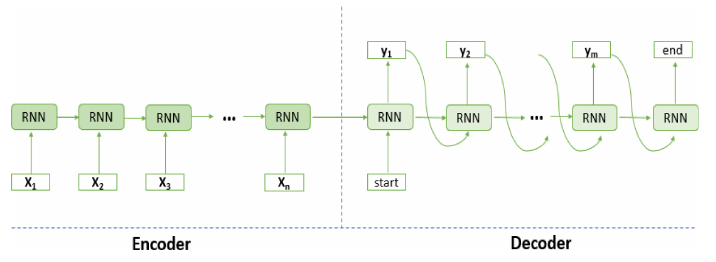
\includegraphics[height=6cm]{encoder_decoder.png}
	\end{center}
	\caption{معماری پایه‌‌ی مدل کدگذار-کدگشا\cite{RL_survey}}
	\label{fig:encoder_decoder}
	\medskip
	\small
\end{figure}

یائو\LTRfootnote{Yao}
و همکاران مدل کدگذاری دوگانه را برای خلاصه‌سازی انتزاعی پیشنهاد داده‌اند. این مدل برای درک بهتر روابط بین متن ورودی و خلاصه مرجع بازنمایی متن ورودی و بازنمایی خلاصه‌ی مرجع را می‌آموزد. همانطور که در شکل \ref{fig:dual_encoder} نشان داده شده است.
%کدگذاری دوگانه به مدل اجازه می‌دهد تا دو نمایش متفاوت از متن را بیاموزد: نمایش متن ورودی و نمایش خلاصه مرجع. این به مدل اجازه می‌دهد تا روابط بین متن ورودی و خلاصه مرجع را بهتر درک کند، که می‌تواند منجر به خلاصه‌های دقیق‌ و حاوی اطلاعات مفید شود.
این مدل از یک کدگذار اولیه، یک کدگذار ثانویه و یک کدگشا مجهز به مکانیزم توجه تشکیل شده است و هر سه ماژول فوق از واحد بازگشتی دروازه‌ای
\LTRfootnote{gated recurrent unit (GRU)}
استفاده می‌کنند. 
کدگذار اولیه بردارهای معنایی هر کلمه در ترتیب ورودی را محاسبه می‌کند. کدگذار ثانویه وزن اهمیت هر کلمه در ترتیب ورودی و بردارهای معنایی مربوطه را دوباره محاسبه می‌کند. در نهایت کدگشا با مکانیسم توجه به صورت مرحله‌ای کدگشایی می‌کند و در هر مرحله یک توالی خروجی با طول ثابت جزئی ایجاد می‌کند. در این مدل کدگذار ثانویه عملیات کدگذاری را براساس ورودی هر مرحله و خروجی مرحله‌ی قبل انجام می‌دهد بنابراین کیفیت متون قبلی تولید شده توسط کدگشا بر خروجی‌های جدید تاثیر می‌گذارد
\cite{yao2018dual}.



\begin{figure}[!h]
	\begin{center}
		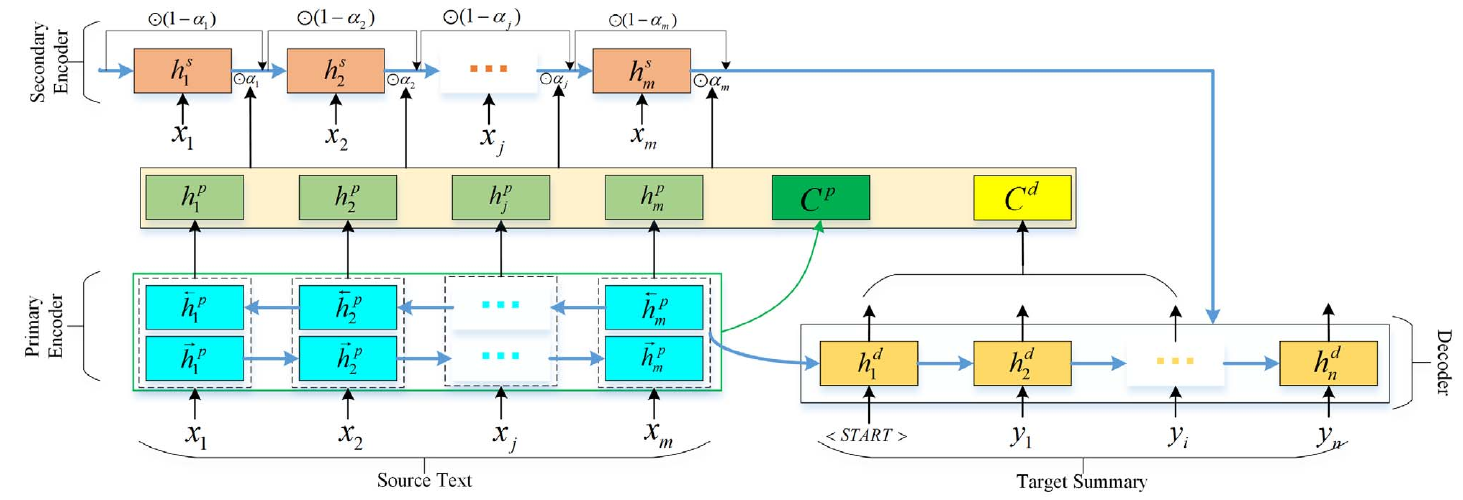
\includegraphics[height=5cm]{dualـencoder.png}
	\end{center}
	\caption{معماری پایه‌‌ی مدل دوگانه‌ی کدگذار 	\cite{yao2018dual}}
	\label{fig:dual_encoder}
	\medskip
	\small
\end{figure}


مدل کدگذاری دوگانه مدل سلسله مراتبی متغیر بر اساس مدل کدگذاری دوگانه برای خلاصه‌سازی متقاطع زبانی\LTRfootnote{cross-lingual}
پیشنهاد شده است. این مدل شامل دو متغیر نهفته محلی و یک متغیر نهفته جامع است. از متغیرهای نهفته محلی برای بازسازی ترجمه و خلاصه زبان مبدأ و از متغیر نهفته سراسری برای تولید خلاصه بین زبانی استفاده می‌شود. قسمت کد گذار این مدل دو بخش دارد که هر بخش وظیفه‌ی تولید یکی از متغیرهای نهفته محلی را دارد و بخش کدگشا با استفاده از نمایش‌های نهفته‌ی محلی خلاصه‌ی نهایی را تولید می‌کند.
ساختار سلسله مراتبی این مدل به آن اجازه می‌دهد تا رابطه سلسله مراتبی بین ترجمه، خلاصه‌سازی و خلاصه‌سازی بین زبانی را بیاموزد\cite{variational}.

\begin{figure}[!h]
	\begin{center}
		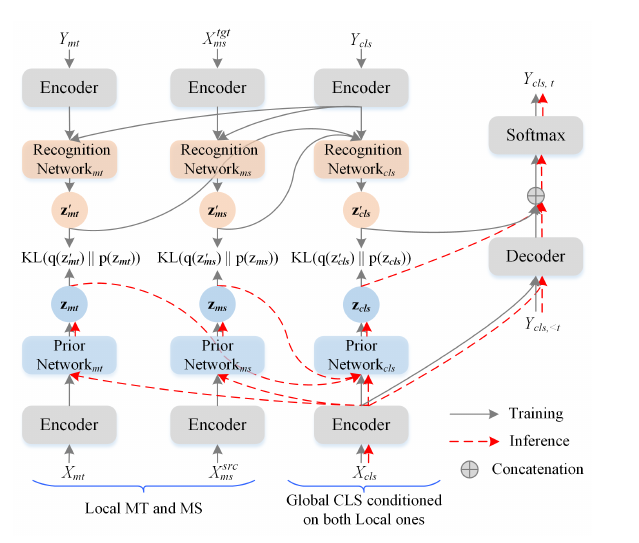
\includegraphics[height=12cm]{Variational Hierarchical Model.png}
	\end{center}
	\caption{معماری پایه‌‌ی مدل سلسله مراتبی متغیر برای خلاصه‌سازی متقابل زبانی\cite{variational}}
	\label{fig:vahie_model}
	\medskip
	\small{
		متغیرهای محلی $ z_mt $ و $ z_ms $ به ترتیب برای ترجمه و خلاصه‌سازی و متغیر جامع $ z_cls $ برای خلاصه‌سازی بین زبانی طراحی شده‌اند. خطوط خاکستری نشان‌دهنده فرآیند آموزشی است که مسئول تولید
		($ z' _{mt} $، $ z'_{ms} $، $ z'_{cls} $)
		از توزیع پسین متناظر پیش‌بینی‌شده توسط شبکه‌ است. خطوط قرمز خط چین نشان دهنده فرآیند استنتاج برای تولید نمایش‌‌های نهفته
		($ z _{mt} $، $ z_{ms} $، $ z_{cls} $)
		از توزیع‌های پیش بینی شده توسط شبکه‌های قبلی است. }
\end{figure}



%\subsection{روش‌های ارايه شده برای متون کوتاه }


%\subsection{روش‌های ارايه شده برای متون طولانی }


\section{روش‌های مبتنی بر مدل ترنسفورمر‌}
با ظهور ترنسفورمرها\LTRfootnote{transformers}
، بهبودهای قابل توجهی در کیفیت نتایج خلاصه‌سازی خودکار به وجود آمد. ترنسفومرها با استفاده از مکانیزم توجه به خود\LTRfootnote{Self-attention}
شباهت بین ورودی‌ها را بدون توجه به موقعیت موازی آن‌ها با حضور مستقل هر توکن در توالی ورودی مدل می‌کنند و به طور مؤثر مشکلات شبکه‌های بازگشتی را حل می‌کنند\cite{vaswani2017attention}. یکی از جهت‌گیری‌های رایج پژوهشی، اصلاح یا تطبیق ترنسفورمرها و مدل‌های زبانی از پیش آموزش دیده با وظایف مختلف مانند خلاصه‌سازی است. مدل‌های مبتنی بر مدل‌های زبانی از پیش آموزش دیده که با هدف خلاصه‌سازی انتزاعی طراحی شده‌اند از ویژگی‌های معنایی و متنی غنی بازنمایی‌های زبان برای بهبود کیفیت و دقت خلاصه‌‌ها استفاده می‌کنند.



پان
\LTRfootnote{Pan}
و همکاران یک مدل خلاصه‌سازی بر اساس مدل برت را پیشنهاد کرده‌اند. نویسندگان استدلال می‌کنند که خلاصه‌های تولید شده توسط مدل‌های خلاصه‌سازی متن موجود که موضوع متن را در نظر نمی‌گیرند، مرتبط یا حاوی اطلاعات مفید نیستند. 
مدل ارائه شده که تی‌برت‌سام\LTRfootnote{T-BERTSum}
نامیده می‌شود از سه بخش ایجاد بازنمایی، مدل موضوعی عصبی\LTRfootnote{Neural Topic Model(NTM)}
و مدل خلاصه‌سازی تشکیل شده است. ساختار مدل را در شکل \ref{fig:tBert_model} نشان داده شده است.
\begin{figure}[!h]
	\begin{center}
		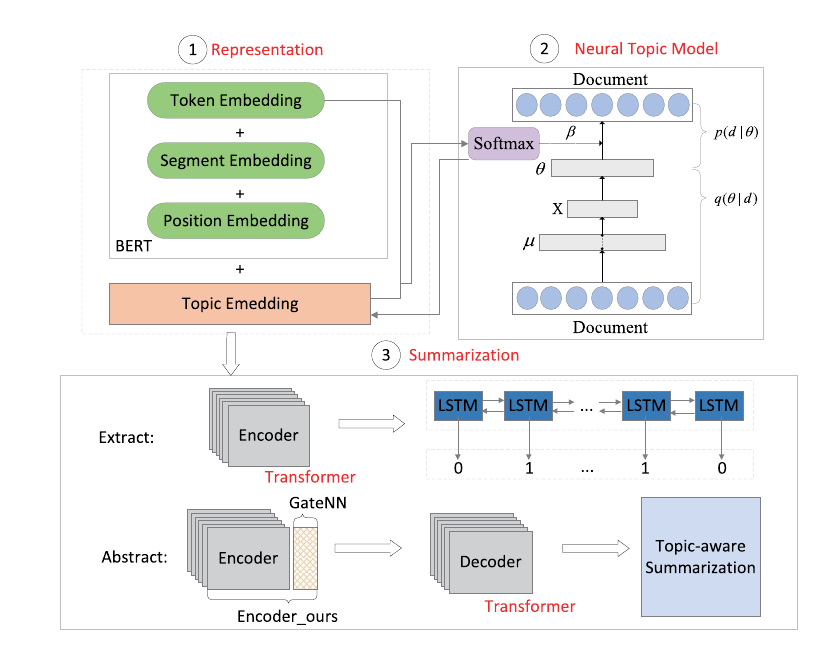
\includegraphics[height=10cm]{tbertsum_framework.png}
	\end{center}
	\caption{معماری مدل تی‌برت‌سام \cite{Ma2022TBERTSumTT}}
	\label{fig:tBert_model}
	\medskip
	\small
\end{figure}



همانطور که در شکل \ref{fig:tBert_embded} نشان داده شده است، بازنمایی ایجاد شده برای هر جمله ورودی، با استفاده از یک شبکه‌ی ترنسفورمر دوسویه‌ی\LTRfootnote{bidirectional}
چند لایه و حاصل جمع چهار نوع تعبیه ( تعبیه نشانه\LTRfootnote{token embedding}
، تعبیه قطعه\LTRfootnote{segment embedding}
، تعبیه موقعیت و تعبیه موضوع) به دست ‌می‌آید که تعبیه موضوع در این مقاله معرفی شده و سه تعبیه دیگر مشابه مدل برت هستند. وجود تعبیه موضوع در تولید بازنمایی هر کلمه یا جمله موجب افزودن اطلاعات پیش زمینه‌ای به هر کلمه و حل مشکل چند معنایی می‌شود.
\begin{figure}[!h]
	\begin{center}
		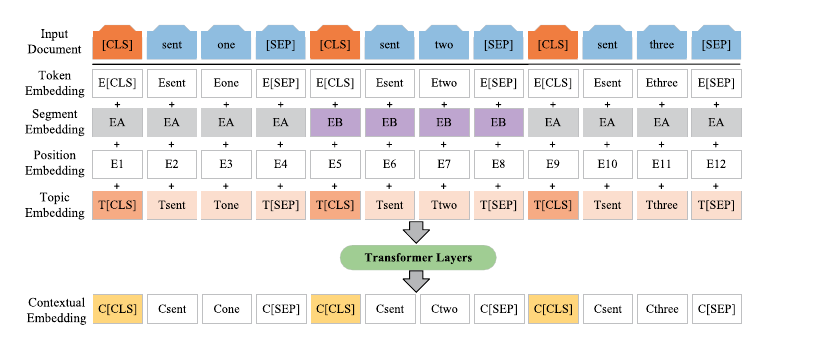
\includegraphics[height=7cm]{TbertSum_embedding.png}
	\end{center}
	\caption{ تعبیه مدل تی‌برت‌سام \cite{Ma2022TBERTSumTT}}
	\label{fig:tBert_embded}
	\medskip
	\small
\end{figure}

مدل موضوعی عصبی وظیفه‌ی ایجاد تعبیه موضوعی را دارد. این مدل دارای دو جزء است: یک شبکه مولد و یک شبکه استنتاج.
شبکه مولد یک سند را به عنوان ورودی می‌گیرد و یک توزیع موضوعی را بر روی کلمات موجود در سند خروجی می‌دهد.
\todo{مفهوم درست نیست}
شبکه استنتاج یک سند را به عنوان ورودی می‌گیرد و خروجی آن پارامترهای توزیع موضوع است. 
بخش خلاصه‌سازی مدل مبتنی بر معماری کدگذار - کدگشای ترنسفورمر است. کدگذار بازنمایی ایجاد شده را به عنوان ورودی می‌گیرد و دنباله‌ای از حالت‌های پنهان را تولید می‌کند. سپس کدگشا با استفاده از  حالت‌های پنهان و متن خلاصه را تولید می‌کند. همانطور که در شکل 
\ref{fig:tBert_transformer}
نشان داده شده است، به منظور فیلتر کردن اطلاعات کلیدی توالی ورودی، شبکه دروازه‌ای قبل از کدگشا اضافه می‌شود.
این شبکه برای کنترل جریان اطلاعات از دنباله ورودی به دنباله خروجی افزوده شده است و باعث می‌شود کدگشا بر روی تولید خلاصه از اطلاعات کلیدی و حذف اطلاعات غیرضروری تمرکز کند. این مدل می‌تواند خلاصه‌هایی تولید کند که مرتبط با موضوع متن و حاوی اطلاعات مفید باشد و قابلیت تطبیق با حوزه‌های مختلف را دارد.
\todo{جمله‌ی اخر تکراری هست}

\begin{figure}[!h]
	\begin{center}
		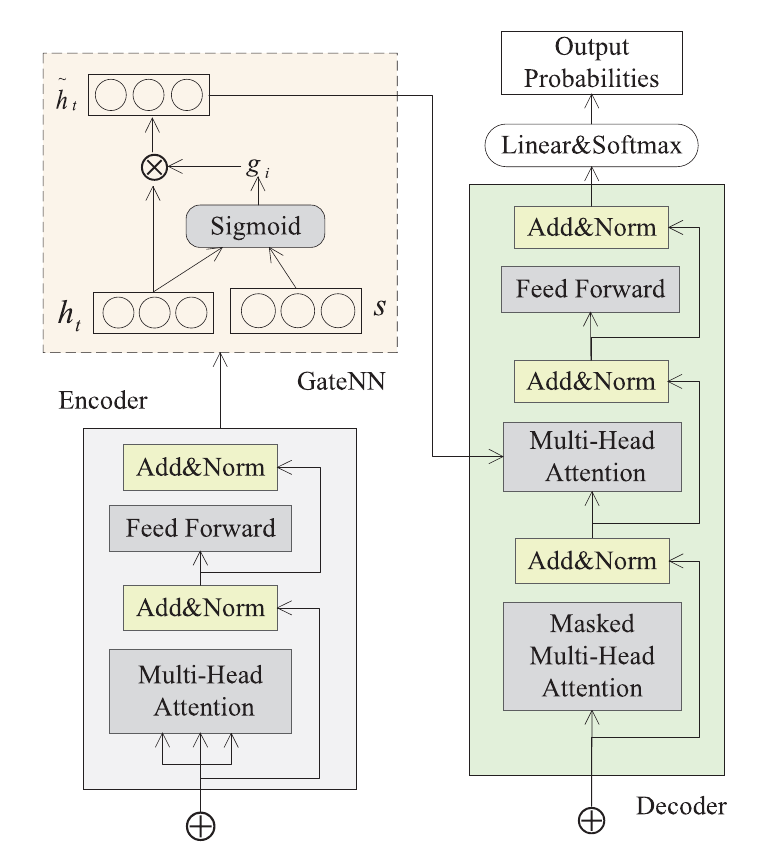
\includegraphics[height=10cm]{tbertsum_transformer.png}
	\end{center}
	\caption{ معماری ترنسفورمر تی‌برت‌سام \cite{Ma2022TBERTSumTT}}
	\label{fig:tBert_transformer}
	\medskip
	\small
	\centerline{	این مدل شامل شبکه‌ی دروازه‌ای و کدگذار-کدگشا با توجه چند سر می‌باشد\cite{Ma2022TBERTSumTT}}
	
\end{figure}
\todo{ادیت}

اکثر مدل‌های خلاصه‌سازی انتزاعی موجود برای تولید خلاصه‌های با طول ثابت طراحی شده‌اند، بنابراین سو
\LTRfootnote{Ming-Hsiang Su}
و همکاران یک مدل دو مرحله‌ای مبتنی بر تنرسفورمر ارائه دادند که خلاصه‌های انتزاعی با طول متغیر را با توجه به تقاضای کاربر تولید کند. مطابق شکل  \ref{fig:two_stage_model}مدل پیشنهادی با تقسیم متن ورودی به بخش‌ها و تولید خلاصه‌ی هر بخش، خلاصه‌ی انتزاعی با طول متغیر تولید می‌کند
\cite{twostage}.
\begin{figure}[!h]
	\begin{center}
		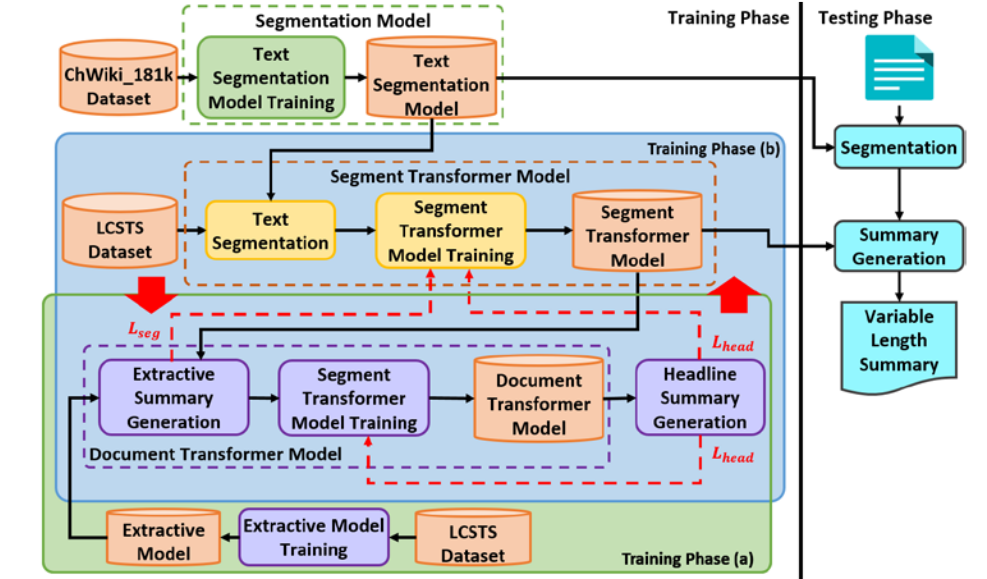
\includegraphics[height=10cm]{two-stage model.png}
	\end{center}
	\caption{ چهارچوب ایجاد خلاصه با طول متغیر\cite{twostage}}
	\label{fig:two_stage_model}
	\medskip
	\small	
\end{figure}

بخش‌‌های مدل ارائه شده به شرح زیر است.
\\
\begin{itemize}
	\item {
		بخش بندی متن: این مرحله متن ورودی را به تعدادی قسمت از پیش تعیین شده تقسیم می‌کند. تعداد بخش‌ها را می‌تواند توسط کاربر مشخص شود یا با توجه به نسبت دلخواه طول ورودی تنظیم کرد.
		برای شناسایی مرزهای بین بخش‌ها از مدل $ BERT-biLSTM $ استفاده می‌شود. این مرحله تضمین می‌کند که مرحله خلاصه‌سازی انتزاعی بر روی بخش‌های منسجم متن انجام می‌شود. هدف این بخش یافتن نقاط تقسیم‌بندی است که نشان دهنده تغییر موضوع در متن است و  به بهبود کیفیت خلاصه‌های تولید شده کمک می‌کند. 
	}
	\item {
		خلاصه‌سازی استخراجی: پس از تقسیم‌بندی متن، با استفاده از یک مدل خلاصه‌سازی استخراجی مبتنی بر برت‌سام
		\LTRfootnote{BertSum}
		مهم‌ترین جمله را از هر بخش استخراج می‌شود.
	}
	\item {
		
	\todo{ادامه‌ی ادیت}	
	}
	
\end{itemize}




خلاصه‌سازی اسناد: در مرحله دوم از جملات استخراج شده برای آموزش ماژول خلاصه‌سازی اسناد استفاده می‌شود. این ماژول یک خلاصه سرفصل از کل ورودی متن ایجاد می‌کند. پارامترهای این ماژول با در نظر گرفتن امتیازات ضرر ماژول خلاصه‌سازی اسناد و ماژول خلاصه‌سازی بخش به روز می‌شود.

خلاصه‌سازی بخش‌ها: بخش‌های به دست آمده از مرحله تقسیم‌بندی متن برای آموزش ماژول خلاصه‌سازی در مرحله اول استفاده می‌شود. این ماژول یک خلاصه بر اساس جمله برای هر بخش تولید می‌کند. امتیازات ضرر ماژول خلاصه‌سازی سند و ماژول خلاصه‌سازی بخش برای به روز رسانی پارامترهای ماژول خلاصه‌سازی بخش در نظر گرفته می‌شود.

آموزش مشارکتی: آموزش مشارکتی برای آموزش متناوب ماژول خلاصه‌سازی بخش و ماژول خلاصه‌سازی اسناد تا زمان همگرایی اعمال می‌شود. این فرآیند به بهینه سازی عملکرد هر دو ماژول کمک می‌کند.

خلاصه‌سازی با طول متغیر: در طول آزمایش، خروجی‌های ماژول خلاصه‌سازی بخش به هم متصل می‌شوند تا نتیجه خلاصه‌سازی انتزاعی با طول متغیر ارائه شود. تعداد بخش‌ها را می‌توان توسط کاربر مشخص کرد یا با توجه به نسبت دلخواه طول ورودی تنظیم کرد.

با ترکیب روش‌های استخراجی و انتزاعی در مدل خلاصه‌سازی دو مرحله‌ای، رویکرد پیشنهادی می‌تواند خلاصه‌های انتزاعی روان و با طول متغیر را با توجه به خواسته‌های کاربر تولید کند.
\todo{ ادیتش کن}
این مدل می‌تواند خلاصه‌های انتزاعی با طول متغیر را با توجه به خواسته‌های کاربر ایجاد کند. این یک پیشرفت نسبت به مدل‌های قبلی است زیرا می‌تواند به طور همزمان به خلاصه‌سازی انتزاعی روان و با طول متغیر دست یابد.






لوئيس و همكاران مدلي با نام بارت 
\LTRfootnote{BART}
ارائه دادند. اين مدل مشابه با مدل اصلي تبديل‌كننده، ساختاري كدگذار-كدگشا دارد. بر خلاف سادگي اين مدل اين مدل را مي‌توان نسخه عمومي‌تري از برت و جي‌پي‌تي 
\LTRfootnote{GPT}
(به دليل داشتن كدگذار دو طرفه و كدگشاي چپ به راست) دانست. (\ref{fig:bart})اين مدل در عمليات توليد متن، مانند ترجمه ماشيني يا خالصه‌سازي انتزاعي متن، و همچنين در فهم متن كاربرد دارد. بارت را می‌توان با استفاده از اهداف رمزگذاری خودکار حذف نویز آموزش داد. در ابتدا، توالی ورودی با استفاده از یک تابع نویز دلخواه خراب می‌شود. سپس ورودی خراب توسط یک شبکه ترنسفورمر بازسازی می‌شود. این مدل طیف گسترده‌ای از نویز ‌ها از جمله پوشاندن توکن، حذف توکن، پر کردن متن، چرخش سند، به هم ریختن جمله (به هم زدن تصادفی ترتیب کلمه یک جمله) را ارزیابی می‌کند\cite{liu2020survey,lewis-etal-2020-bart}. 
\todo{یک کم دیگه اضافه کن}
\begin{figure}[!h]
	\begin{center}
		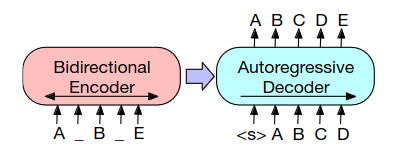
\includegraphics[height=4cm]{bart.png}
	\end{center}
	\caption{ ساختار مدل بارت \cite{lewis-etal-2020-bart}}
	\label{fig:bart}
	\medskip
	\small
	ورودی‌های کدگذار نیازی به همسویی با خروجی‌های کدگشا ندارند، که امکان تبدیل نویز دلخواه را فراهم می‌کند. در اینجا، یک سند با جایگزین کردن دهانه‌های متن با نمادهای ماسک خراب شده است. سند خراب (سمت چپ) با یک مدل دو طرفه کدگذاری می‌شود و سپس احتمال سند اصلی (سمت راست) با کدگشای خودبازگشتی محاسبه می‌شود. برای تنظیم دقیق، یک سند خراب به رمزگذار و رمزگشا وارد می‌شود و ما از نمایش‌هایی از حالت پنهان‌ نهایی کدگشا استفاده می‌کنیم\cite{lewis-etal-2020-bart}.
\end{figure}


با اين كه بارت دقت خلاصه‌سازی انتزاعي متن را بهبود بخشيد، ولي عمل‌هاي تعریف شده در مرحله پيش‌آموزش آن، مختص خلاصه‌سازی انتزاعي متن نبودند، در نتیجه در سال 2020 مدلي تحت عنوان پگاسوس 
\LTRfootnote{PEGASUS}
توسط ژنگ و همكاران ارائه شد كه معماري مشابه با بارت داشت ولي پيش‌آموزش آن مختص خلاصه‌سازی انتزاعي متن بود.
مدل پگاسوس
یک مدل دنباله به دنباله کدگذار کدگشا مبتنی بر ترنسفورمر است که بر روی مجموعه‌های متنی بدون نظارت با هدف تولید جملات فاصله‌افتاده
\LTRfootnote{‫‪gap‬‬ ‫‪sentences‬‬ ‫‪generation‬‬}
از قبل آموزش داده شده است
\cite{zhang2020pegasus}.

این مدل دو عمل پيش‌آموزش معرفي كرده است كه در ادامه به شرح آنها مي‌پردازيم:
\begin{enumerate}
	\item {
		توليد جملات فاصله‌افتاده : اين فرض مطرح شده است كه اگر عمل پيش‌آموزش مدل به وظایف
		پايين‌دست 
		\LTRfootnote{downstream task}
		نزديك‌تر باشد، نتیجه نهايي بهتر و همچنين تنظیم دقیق پارامترها
		\LTRfootnote{fine-tuning}
		سريع‌تر خواهد بود. با توجه به اين كه اين مدل قرار است فقط براي خلاصه‌سازی انتزاعي متن استفاده شود، عمل
		پيش‌آموزش توليد متن‌هاي مشابه با خلاصه از يك سند ورودي تعریف شده‌است. بر اساس يك
		متغیر كه درصد جملات پنهان‌شده را مشخص مي‌شود، تعدادي از جملات انتخاب شده و هر جمله
		به طور كامل با توكن $ [MASK1] $ جايگزين ميشود. براي انتخاب اين جملات، سه راه پيشنهاد
		شده است.
		\begin{itemize}
			\item {
				انتخاب تصادفي: $ m $جمله به صورت تصادفي از متن انتخاب شده و پنهان مي‌شوند.
			}
			\item{
				انتخاب جملات اول متن: $ m $جمله اول متن پنهان مي‌شوند. دليل اين كار، فرض مهم‌تر
				بودن جملات ابتداي متن نسبت به جملات بعدی است.
			}
			\item{
				انتخاب جملات مهم متن: براي انتخاب $ m $ جمله مهم متن از تقريب معيار ارزيابي روژ-۱
				استفاده می‌شود. به ازای هر
				جمله از متن، يك دوتايي از آن جمله و كل متن سند فاقد آن جمله ساخته شده و ارزيابي
				مي‌شود كه چقدر ممکن است اين جمله، خلاصه كل سند فاقد آن جمله باشد. جملاتي
				كه امتیاز بالاتر گرفته‌اند از نظر خلاصه بودن مهم‌تر هستند و پنهان می‌شوند.
			}
			
			
		\end{itemize}
	}
	{ مدل زباني پوشيده شده: مشابه مدل برت ۵۱ درصد از توكن‌هاي متن ورودي انتخاب
		مي‌شوند و سپس 80 درصد از اين توكن‌ها، با توكن $ [MASK2] $ و10 درصد توكن‌ها با يك توكن
		تصادفي جايگزين می‌شوند. 10 درصد ديگر بدون تغيير باقي می‌ماند.
		شكل \ref{fig:pegasus} اعمال همزمان اين دو عمل، يعني توليد جمالت فاصله افتاده و مدل زباني پوشيده شده
		را بر روي يك مثال نشان می‌دهد.
	}
\end{enumerate}

\begin{figure}[!h]
	\begin{center}
		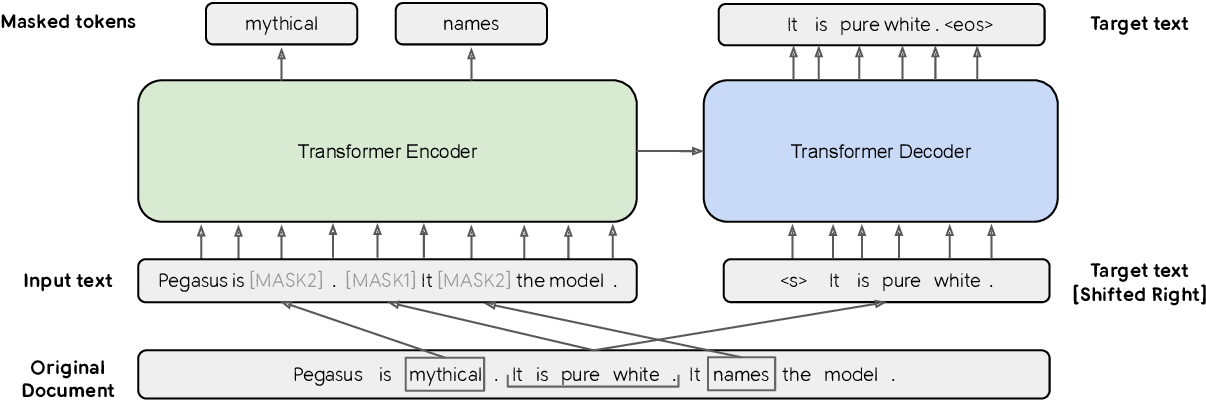
\includegraphics[height=5cm]{pegasus.png}
	\end{center}
	\caption{ ساختار مدل پگاسوس \cite{zhang2020pegasus}}
	\label{fig:pegasus}
	\medskip
	\small{
		معماری پایه پگاسوس یک کدگذار-کدگشا ترنسفورمر استاندارد است. جملات فاصله‌افتاده و مدل زبانی پوشیده شده به طور همزمان در این مثال به عنوان اهداف پيش‌آموزش اعمال می‌شوند. در اصل سه جمله وجود دارد. یک جمله با $ [MASK1] $ پوشانده شده و به عنوان متن تولید هدف جملات فاصله‌افتاده استفاده می‌شود. دو جمله دیگر در ورودی باقی می‌مانند و برخی از نشانه‌ها به طور تصادفی توسط$ [MASK2] $پوشانده می‌شوند
		\cite{zhang2020pegasus}.}
\end{figure}

کدیا
\LTRfootnote{Kedia}
و همکاران الگوریتم حداکثر سازی نقطه-محصول فرا یادگیری (ام‌دات)
\LTRfootnote{Meta-Learned Dot-Product Maximization (MDot)}
را پیشنهاد دادند. این الگوریتم بر اساس ایده به حداکثر رساندن حاصل‌ضرب نقطه‌ای بین گرادیان‌های مدل در نقاط مختلف آموزش با استفاده از تکنیکی به نام تفاوت‌های محدود
\LTRfootnote{finite differences}
است. این الگوریتم از نظر محاسباتی کارآمد است و می‌تواند برای مدل‌های بزرگ مانند برت اعمال شود و سربار محاسباتی را کاهش بدهد
\cite{sherborne2023meta}.
عملکرد مناسب مدل پگاسوس در خلاصه‌سازی متون باعث شده بهترین مدل خلاصه‌سازی متون کوتاه مبتنی بر مدل پگاسوس و تکنیک تنظیم 
\LTRfootnote{regularization}
ام‌دات باشد.

\begin{figure}[!h]
	\begin{center}
		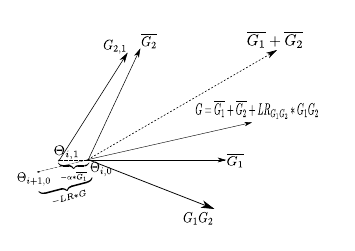
\includegraphics[height=6cm]{Mdot.png}
	\end{center}
	\caption{ الگوریتم ام‌دات \cite{sherborne2023meta}}
	\label{fig:Mdot}
	\medskip
	\small{
		محاسبه گرادیان برای به حداکثر رساندن محصول نقطه‌ای با استفاده از تقریب تفاضل محدود، و استفاده از آن برای تنظیم گرادیان استاندارد
		\cite{sherborne2023meta}.
	}
\end{figure}


%\section{روش‌های مبتنی بر مدل‌های از پیش آموزش دیده}



\subsection{ایده‌های ارائه شده بهبود خلاصه‌سازی متون طولانی }


یکی از مشکلات مدل ترنسفومر در خلاصه‌سازی متون طولانی حافظه‌ی درجه دوم پیچیدگی‌های محاسباتی و تعداد زیاد عملیات می‌باشد. برای حل این مشکلات کار‌های مختلفی انجام شده است. به عنوان مثال شبکه‌ی ریفورمر
\LTRfootnote{‫‪Reformer‬‬}
برای حل چالش‌های محاسباتی مرتبط با پردازش دنباله‌های طولانی متن ارائه شده است. لایه‌های برگشت‌پذیر
\LTRfootnote{reversible layers}
معرفی شده در این مقاله امکان بازسازی ورودی از خروجی را در طول گذر به عقب، کاهش نیازهای حافظه و امکان پردازش کارآمد دنباله‌های طولانی را فراهم می‌کنند.
. علاوه بر این، ریفورمر از تکه تکه کردن برای پردازش بخش‌های کوچک تر ورودی به طور مستقل استفاده می‌کند که موازی‌سازی را ممکن می‌کند و مصرف حافظه را کاهش می‌دهد. یکی از کمک‌های کلیدی آن استفاده از درهم‌سازی حساس به مکان 
\LTRfootnote{‫‪locality-sensitive‬‬ ‫‪hashing‬‬ ‪(LSH‬)}
 در مکانیسم توجه
است. درهم‌سازی حساس به مکان با توجه به زیرمجموعه‌ای از نشانه‌ها بر اساس مقادیر هش آنها، محاسبه توجه کامل را تقریب می‌زند، که منجر به محاسبه توجه کارآمدتر می‌شود. علاوه بر این، ریفورمر از کدگذاری‌های موقعیت محوری برای کدگذاری اطلاعات موقعیت توکن‌ها به صورت فشرده استفاده می‌کند. این تکنیک‌ها مجموعاً مدل ریفورمر را بسیار مقیاس‌پذیر و کارآمد در حافظه می‌سازد، و آن را قادر می‌سازد تا دنباله‌های طولانی متن را مدیریت کند و در عین حال عملکرد رقابتی را در وظایف مختلف پردازش زبان طبیعی حفظ کند
\cite{reformer}
\todo{ادیت}

. همچنین شبکه‌ی ترنسفورمر پراکنده 
\LTRfootnote{sparse }
با معرفی فاکتورسازی‌ ماتریس پراکنده‌ی توجه، زمان و حافظه مورد نیاز را به کاهش می‌دهد.
با استفاده از پراکندگی، مدل می‌تواند تنها به زیرمجموعه‌ای از نشانه‌های ورودی توجه کند و روی مرتبط‌ترین اطلاعات تمرکز کند و بقیه را نادیده بگیرد. این رویکرد پیچیدگی محاسباتی را کاهش می‌دهد و مدل می‌تواند توالی‌های طولانی‌تر را مدیریت کند\cite{child2019generating}. مشابه شبکه‌ی ترنسفورمر پراکنده مدل بیگ‌برد نیز
\LTRfootnote{‫‪Big‬‬ ‫‪Bird‬‬}
با استفاده از مکانیزم توجه پراکنده
\LTRfootnote{‫‪Sparse‬‬ ‫‪attention‬‬}
که وابستگی را به خطی کاهش ‌می‌دهد و عملکرد ترنسفورمر را در مواجه با دنباله‌ی کلمات
%\LTRfootnote{‫‪sequence‬‬}
طولانی بهبود می‌بخشد. مدل بیگ‌برد نوآوری‌های دیگری مانند توجه جامع
\LTRfootnote{global attention}
را معرفی می‌کند، که در آن توکن‌های خاص به تمام توکن‌های دیگر در دنباله توجه می‌کنند و وابستگی‌های دوربرد را به طور موثرتری به دست می‌آورند. همچنین شامل یک فرآیند پالایش تکراری است که وزن‌های توجه را برای بهبود عملکرد مدل اصلاح می‌کند
\cite{zaheer2020big}. 
\todo{ادیت}


%ژیائو و کارنی \LTRfootnote{‫Xiao \& ‬‬ ‫‪Carenini‬‬} با تمرکز برکاهش تکرار و افزونگی در خلاصه‌سازی اسناد طولانی مدلی طراحی کرده‌اند که کدگشایی آن براساس مکانیزم توجه آگاه از افزونگی می‌باشد. علاوه بر این تابع ضرر \LTRfootnote{‫‪Loss‬‬ ‫‪function‬‬} طراحی کرده‌اند که برای تعادل بین اهمیت و افزونگی مناسب باشد. این روش باعث انتخاب جملات مهم و غیر زائد می‌شود \todo{دوباره بنویس} \cite{xiao2020systematically}

در سال‌های اخیر مدل‌های مختلفی برای بهبود کیفیت خروجی مدل خلاصه‌سازی خودکار اسناد بلند ارائه شده است. به عنوان مثال پایل
\LTRfootnote{‫‪Pilault‬‬}
و همکاران که برای بهبود خلاصه انتزاعی نهایی متون طولانی از رویکرد ترکیبی استخراجی-انتزاعی با استفاده از مدل زبانی از پیش آموزش دیده جی‌پی‌تی-دو
\LTRfootnote{GPT-2}
استفاده می‌کنند. در این مدل مرحله استخراج ساده قبل از تولید خلاصه انجام می‌شود، سپس برای شرطی کردن مدل زبانی ترنسفورمر بر روی اطلاعات مربوط قبل از تولید خلاصه استفاده می‌شود. این رویکرد در مقایسه با کارهای قبلی که از مکانیزم کپی استفاده می‌کنند، خلاصه‌های انتزاعی بیشتری تولید می‌کند
\cite{pilault2020extractive}. 
پانگ
\LTRfootnote{Pang}
و همکاران یک ساختار سلسله مراتبی برای اسناد طولانی فرض کرده‌اند. در این ساختار سطح بالا بر وابستگی دوربرد تمرکز می‌کند و سطح پایین جزئیات را حفظ می‌کند. 
در استنتاج از پایین به بالا، تعبیه‌های متنی نشانه‌ها با استفاده از توجه محلی محاسبه می‌شوند و برای دریافت وابستگی‌های دوربرد و زمینه جامع، استنتاج از بالا به پایین برای نمایش‌های توکن اعمال می‌شود. یک ساختار پنهان چند مقیاسی دو سطحی استفاده می‌شود، که در آن سطح پایین شامل نمایش‌های نشانه‌ای است که توسط استنتاج پایین به بالا محاسبه می‌شود، سپس با اعمال مکانیزم توجه به سطوح بزرگ‌تر روابط بین بخش‌های مختلف سند را بدست می‌آورد. ساختار مدل را در شکل \ref{fig:top_down} نشان داده شده است. روش پیشنهادی یک رویکرد جدید امیدوارکننده برای خلاصه‌سازی اسناد طولانی است و نسبت به روش‌های قبلی کارآمدتر و موثرتر است\cite{pang2023long}.
% این چارچوب استنتاج از پایین به بالا را با استنتاج از بالا به پایین برای بهبود استنتاج نمایش توکن هم‌افزایی می‌کند 

\begin{figure}[!h]
	\begin{center}
		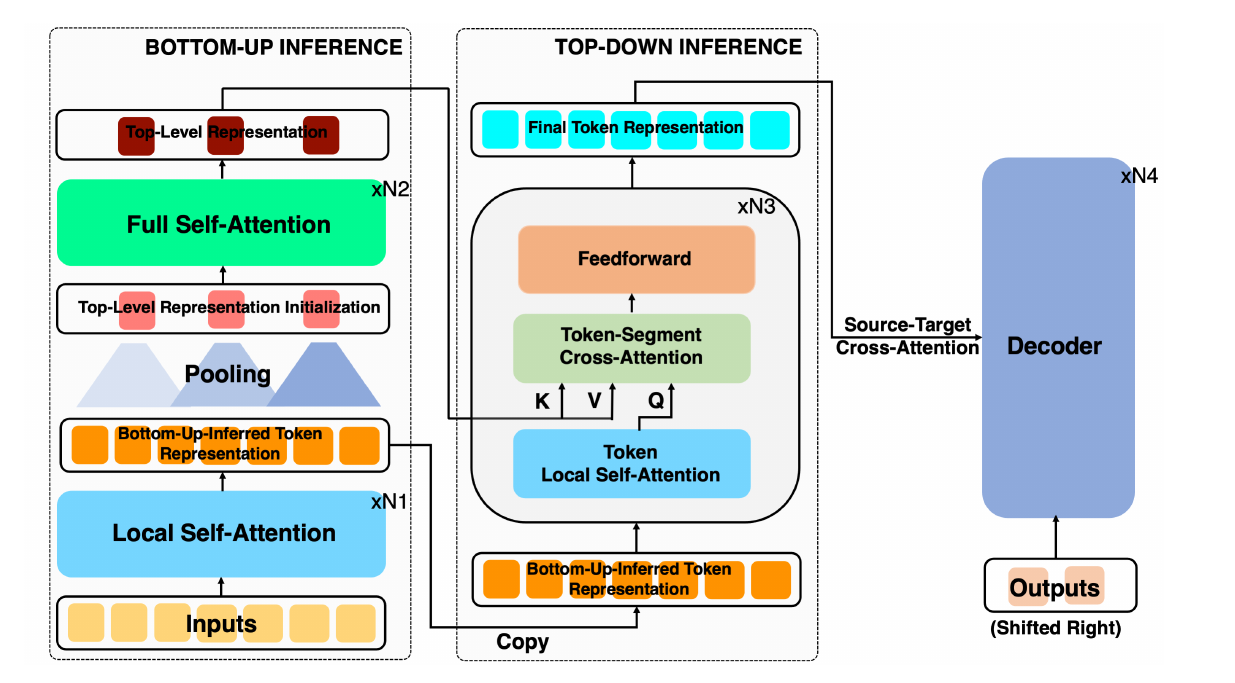
\includegraphics[height=8cm]{top_down.png}
	\end{center}
	\caption{ معماری مدل ترنسفورمر از بالا به پایین\cite{pang2023long}}
	\label{fig:top_down}
	\medskip
	
\end{figure}


%. روش پیشنهادی یک رویکرد جدید امیدوارکننده برای خلاصه‌سازی اسناد طولانی است و بهترین عملکرد در خلاصه‌سازی متون طولانی را دارد
\todo{ادیت}

جیدیوتیس و همکاران شیوه‌ی تقسیم و غلبه ( دنسر) 
\LTRfootnote{Divide-and-ConquER (DANCER)}
را برای بهبود خلاصه‌سازی اسناد طولانی پیشنهاد کرده اند.این روش به طور خودکار خلاصه یک سند را به چند بخش‌ تقسیم می‌کند و هر یک از این بخش‌ها را به بخش مناسب سند جفت می‌کند تا خلاصه‌های هدف متمایز ایجاد کند. شیوه‌ی معرفی شده در نظر می‌گیرد که متون طولانی به صورت بخش‌های گسسته ساختاربندی شده‌اند. 

برای مطابقت هر قسمت از خلاصه با بخشی از سند در دنسر از معیار روژ 
\LTRfootnote{ROUGE}
استفاده ‌می‌شود. در این روش معیار روژ-ال بین هر یک از جملات خلاصه و تمام جملات سند محاسبه می‌شود و هر جمله‌ی خلاصه هدف به بخش حاوی جمله با بیشترین روژ- ال نسبت داده می‌شود. 
سپس تمام جملات خلاصه‌ی هدف مربوط به هر بخش را به هم الحاق می‌کنیم تا خلاصه‌ی هدف برای هر بخش ایجاد شود. در طول آموزش هر بخش از سند به همراه جمله‌ی خلاصه‌ی مربوط به آن به عنوان متن ورودی و خلاصه‌ی هدف استفاده می‌شود. 
مزایای این روش آموزش:
\begin{enumerate}
	\item {
		تقسیم مساله به چند زیر مساله باعث کاهش پیچیدگی و ساده‌سازی مساله می‌شود.
	}
	\item {
		انتخاب خلاصه‌های هدف برای هر بخش بر اساس امتیازات روژ-ال هر جمله باعث تطابق بهتر و متمرکزتر بین دنباله‌های منبع و هدف ایجاد می‌شود.
	}
	\item {
		تقسیم هر سند آموزشی به چند جفت ورودی-هدف، نمونه‌های آموزشی بسیار بیشتری ایجاد می‌کند. این کار برای مدل‌های خلاصه‌سازی عصبی مفید است. 	
	}
	\item {
		این روش می‌تواند از مدل‌های خلاصه‌سازی مختلف از جمله شبکه‌ی عصبی بازگشتی و ترنسفورمرها استفاده کند.
	}
\end{enumerate}


هنگام کار با اسناد ساختاریافته طولانی، معمولاً همه بخش‌های سند کلیدی برای سند نیستند. اگر یک مقاله آکادمیک را به عنوان مثال در نظر بگیریم، بخش‌هایی مانند مرور ادبیات یا پیشینه در تلاش برای خلاصه کردن نکات اصلی مقاله ضروری نیستند و باعث افزودن نویز می‌شوند. بنابراین از بخش مرور ادبیات صرف نظر می‌شود و تمرکز سیستم خلاصه‌سازی فقط روی بخش‌های مقدمه، روش‌ها، نتایج و نتیجه‌گیری می‌باشد.
\todo{میتونه حذف بشه }

این مدل قابل ترکیب با پگاسوس یا مدل مولد نقطه‌ای 
\LTRfootnote{Pointer-Generator model}
می‌باشد.
بخش کدگشا مدل مولد نقطه‌ای با ایجاد جملات تکراری مقابله ‌می‌کند.
هرچند ممکن است به خاطر تکرار اطلاعات در بخش‌های مختلف بازهم خلاصه‌ی تکراری ایجاد شود.

شیونگ و همکاران با اصلاح هدف بهینه‌سازی، معماری مدل‌‌های از پیش آموزش دیده و مجموعه‌ی دادگان پیش‌آموزش
\LTRfootnote{pretraining corpus}
روشی را برای ساخت مدل‌های مناسب متون طولانی پیشنهاد می‌کنند. مدل‌های پيش‌آموزش دیده متن به متن، مانند برت و بارت، معمولاً بر روی دنباله‌های متن کوتاه، مانند جملات یا پاراگراف‌ها آموزش داده می‌شوند. در حالی که بسیاری از وظایف پردازش زبان طبیعی، مانند پاسخگویی به سؤال و خلاصه کردن، به توانایی پردازش توالی متن طولانی نیاز دارند این مقاله تعدادی از تکنیک‌ها را برای تطبیق مدل‌های متن به متن از پیش آموزش دیده برای دنباله‌های متن طولانی پیشنهاد می‌کند. این تکنیک‌ها عبارتند از:
\begin{itemize}
	\item{
		ارائه‌ی مدل براساس یک ترنسفورمر با 	مکانیزم توجه به خود پراکنده‌ی بلوکی
		\LTRfootnote{Block-sparse self-attention}
		در قسمت کدگذار است. این مکانیزم امکان استفاده‌ی مجدد از وزن‌های مدل‌های از پیش آموزش دیده را فراهم می‌کند.	
	}
	
	\item {
		مکانیرم توکن سراسری
		\LTRfootnote{Global-token mechanism}:
		در این مکانیزم یک مجموعه‌ی کوچک از توکن‌های سراسری به کل توالی توجه می‌کنند و امکان تعاملات دوربرد در کدگذار فراهم می‌شود.
	}
	\item{
		هم‌پوشانی بلوک‌های توجه
		\LTRfootnote{ Overlapping attention windows}
		: توجه لغزشی با همپوشانی یک راه ساده برای معرفی اتصالات دوربرد در مدل‌های توجه محلی است. در این رویکرد، توکن‌های درون هر بلوک به تمام توکن‌های درون خود بلوک و همچنین نیمی‌از توکن‌های بلوک‌های چپ و راست مجاور نزدیک می‌شوند. این نسخه بلوکی از پنجره‌های توجه همپوشانی، راه ساده‌تر و کارآمدتری را برای معرفی اتصالات دوربرد ارائه می‌کند و در عین حال موازی‌سازی را در پیاده‌سازی مدل تسهیل می‌کند.
		
	}
	\item{
		لایه‌ی خود توجه مبتنی بر ادغام بلوکی تقویت شده
		\LTRfootnote{Pooling-augmented blockwise attention}:
		این لایه به عنوان جایگزین لایه خود توجهی برای اتصالات دوربرد معرفی شده است. این رویکرد به واحدهای توجه درون بلوک‌ها اجازه می‌دهد تا به جای توجه به همسایگان بلافصل خود، بر خلاصه‌ای از اطلاعات کلی در بلوک‌ها تمرکز کنند. این لایه در تصویر \ref{fig:attention_pooling}نشان داده شده است. این مدل را قادر می‌سازد تا از اطلاعات گسترده تری در سراسر سند برای تصمیم گیری استفاده کند و وابستگی‌های دوربرد را در نظر بگیرد. با بکارگیری عملیات ادغام، ابعاد و نمایش بردارهای توجه کاهش می‌یابد که منجر به افزایش سرعت و کارایی مدل می‌شود.}
\end{itemize}
نویسندگان تکنیک‌های پیشنهادی را در تعدادی از وظایف توالی متن طولانی، از جمله پاسخ‌گویی به سؤال و خلاصه‌نویسی، ارزیابی کرده‌اند. نتایج نشان می‌دهد که مدل‌های اقتباس‌شده در تمامی‌وظایف از مدل‌های پایه بهتر عمل می‌کنند.
این تکنیک‌ها استفاده از مدل‌های متنی از پیش آموزش دیده را برای طیف وسیعی از وظایف پردازش زبان طبیعی ممکن می‌سازد
\cite{Xiong2022AdaptingPT}.
\begin{figure}[!h]
	\begin{center}
		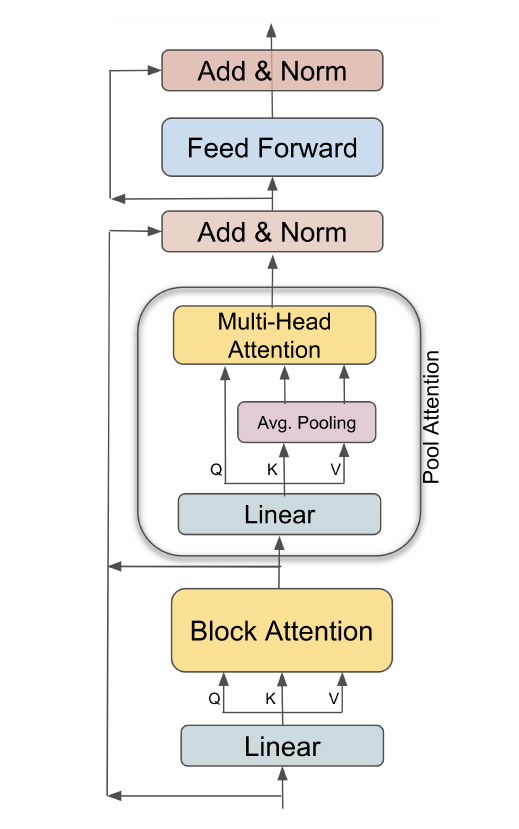
\includegraphics[height=8cm]{pooling_attention.png}
	\end{center}
	\caption{ لایه خودتوجهی تقویت شده ادغام شده \cite{Xiong2022AdaptingPT}}
	\label{fig:attention_pooling}
	\medskip
	\small
\end{figure}













